To test the described method for inferring functional connectivity from calcium imaging data, we simulated a network of stochastically connected neurons constructed as close as possible to resemble the real cortical microcircuits, based on experimental data available from the literature \cite{Braitenberg1998, Urquijo2000, Lefort2009, Sayer1990}.  We prepared sparse random networks of $N=10-500$ neurons. Each neuron was modeled using Eqs. \eqref{eqn:glm:definition} and \eqref{eqn:h:definition}.

The network was divided into excitatory (80\%) and inhibitory (20\%) neurons \cite{Braitenberg1998, Urquijo2000}, each respecting Dale's law, i.e., all axons for a particular neuron were either excitatory or inhibitory (corresponding to all positive or all negative columns in our functional connection weight matrix, $\bw$). Neurons were randomly connected to each other with probability $0.1$ \cite{Braitenberg1998, Lefort2009} XXX this isn't strictly true, is it? XXX.  Synaptic weights for excitatory connections, as defined by EPSP peak amplitude, were randomly drawn from exponential distribution with the mean of $0.5 \mu V$ \cite{Lefort2009, Sayer1990}. These were then converted to GLM weights: while synaptic weights physiologically were measured in $\mu V$, in GLM functional connectivity weights were measured in log-rate units of Eq. \eqref{eqn:glm:definition}). GLM weights described the change in the probability of the neuron $i$ to fire given neuron $j$ had fired before, as opposed to physiologically measured injected currents or changes in membrane potential. By utilizing this definition, synaptic weights were converted into GLM weights assuming that each EPSP corresponded to added probability of neuron spiking in given time bin of $\Delta P = V_E/V_{b}$, where $v_E$ is peak EPSP amplitude and $V_b$ is the membrane resting potential below threshold (implying that $V_{b}/V_E$ EPSPs would be required to trigger neuron over the threshold), 

\begin{equation}\label{eqn:convert}
\w_{ij}=\ln(-\ln(e^{-r_i\tau_w}-V_E/V_{b})/r_i\tau_w), 
\end{equation}

\noindent where $r_i=\exp(b_i)$ is the base firing rate of neuron $i$ and $\tau_w=10$ msec was the typical EPSP/IPSP scale over which single EPSP affects the firing probability of the neuron $i$.  %For small $r_i\tau_w$ this could be replaced with
% 
% \begin{equation}\label{eqn:convert-smalldt}
% \w_{ij}=\ln\left(1+\frac{V_E/V_{b}}{r_i\tau_w}\right).
% \end{equation}

Inhibitory connections were also drawn from exponential distribution with the negative mean. Inhibitory connections strength was chosen so as to balance excitatory and inhibitory currents in the network and achieve an average firing rate of  $\approx 5 $ Hz. Practically, the mean strength of inhibitory connections was about 10 times larger than that of the excitatory connections. 

The time course of functional connectivity weights $\w_{ij}(t)$ was modeled as the difference of two exponentials with the rise time of 1 msec and decay time of 10 msec for excitatory and 20 msec for inhibitory currents \cite{Sayer1990}. Up to 25\% variation in these time constants could be allowed. We neglected conduction delays, given that the time delay below $\sim 1$ msec expected in local cortical circuit was smaller than the time step of our computer simulation.  Additionally to excitatory and inhibitory currents, each neuron was modeled to have refractory current with the time-course described as an exponential with time constant of 10 ms.

Spike-trains were generated using GLM by simulating network forward in time with the time step of 1 ms.  Given the spike rasters, the fluorescence observations were generated using calcium dynamics model Eq. \eqref{eqn:ca:definition}. Parameters for the model were chosen according to our experience with few actual cells analyzed using algorithm of \cite{Vogelstein2009}, see Table \ref{table:caparm}.  The population of cells was generated with these parameters allowing cell-to-cell variance of at least 30\%. XXX explain in more detail the distribution from which all the parameters were taken, something like a uniform distribution with bounds based on data.  add to table below the bounds too.  photon budget should be in terms of the actual parameters of our model XXX Fluorescence was obtained for calcium imaging at the frame-rate of 33 Hzor 66Hz.  From 300 sec to 3600 sec of calcium imaging data was simulated.

\begin{table}[h!b!p!]
\caption{Table of simulation parameters.}\label{table:caparm}
\begin{tabular}{ll}
\hline
Total neurons & 10-500 \\
Excitatory neurons & 80\% \\
Connections sparseness & 10\% \\
Baseline firing rate & 5  Hz\\
Mean EPSP strength & 0.5 $\mu$V \\
Mean IPSP strength & 2.3 $\mu$V\\
EPSP profile & 1 msec rise time, 10 msec decay time \\
IPSP profile & 1 msec rise, 20 msec decay time \\
\hline
Mean Ca noise $\sigma_c$ & 28 $\mu$M \\
Mean Ca jump $A_c$ & 80 $\mu$M \\
Mean Ca background $C_b$ & 24 $\mu$M \\
Mean Ca decay time $\tau_c$ & 0.25 sec \\
Mean photon budget $\alpha_c$ & 1-80 Kph/neuron/frame \\
$K_d$ & 200 $\mu$M \\
\hline
\end{tabular}
\end{table}

\begin{figure}
\centering
\begin{minipage}[c]{0.49\hsize}
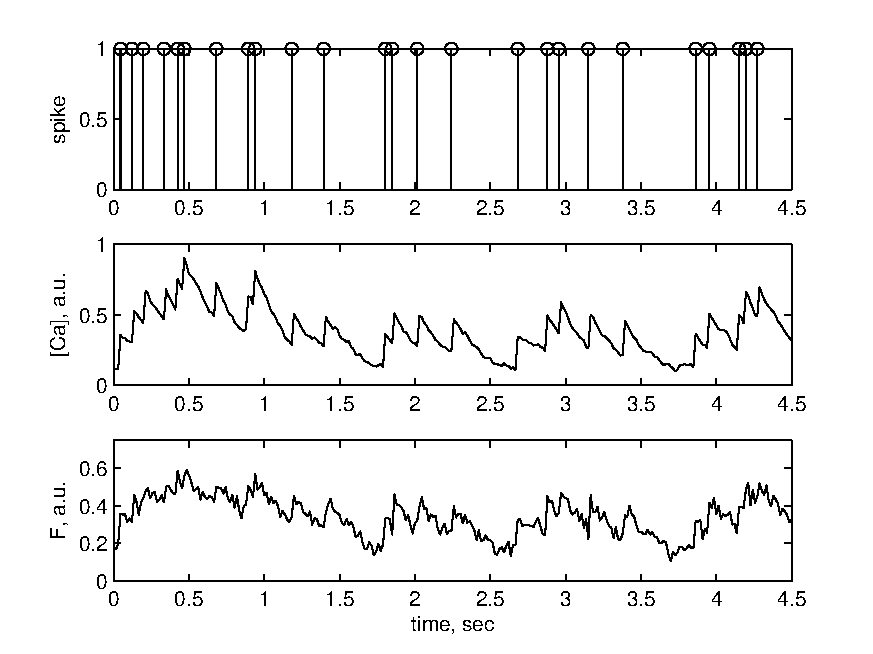
\includegraphics[width=\hsize]{../figs/Figure0b_fluor_eg_hlowSNR}
\end{minipage}
\begin{minipage}[c]{0.49\hsize}
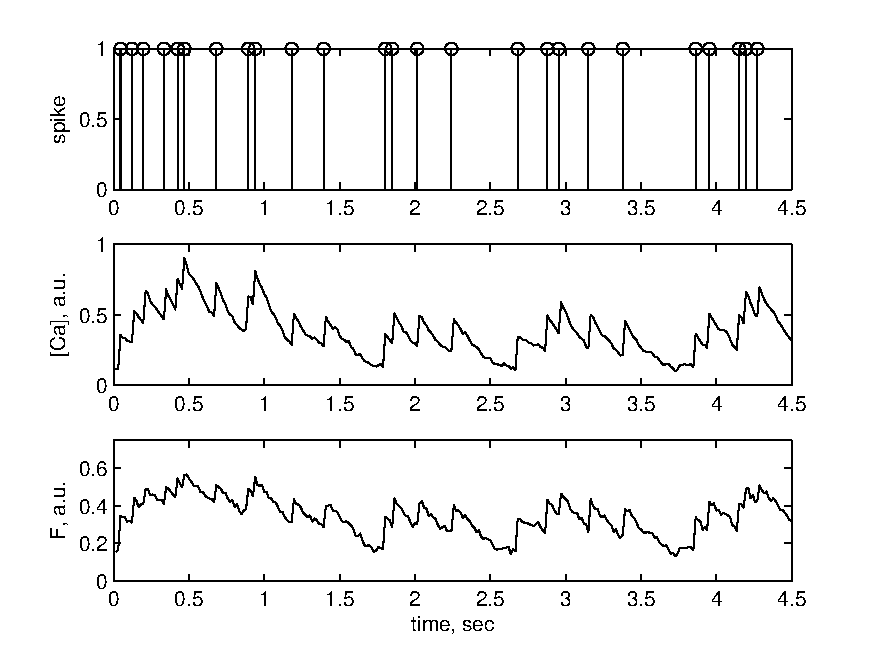
\includegraphics[width=\hsize]{../figs/Figure0a_fluor_eg_highSNR}
\end{minipage}
\caption{Examples of calcium and fluorescence traces for low (photon budget 5 Kph/neuron/frame, left)
and high SNR regimes (photon budget 40 Kph/neuron/frame, right). XXX J will modify to have real data. XXX}
\label{fig:egfluor}
\end{figure}
